\subsection{Activities}
%%%%%%%%%%%%%%%%%%%%%%%%%%%%%%%%%%%%%%%%%%%%%%%%%%%%%%%%%%%%%%%%%%%%%%

\subsubsection{Refinements to the threaded code}
\begin{itemize}
	\item Scheduling policies for POSIX threads were studied in more detail and some portions of the code were fixed.
	\item Added command line interface to the program to set these options.
	\item This code has not been tested yet.
\end{itemize}

%%%%%%%%%%%%%%%%%%%%%%%%%%%%%%%%%%%%%%%%%%%%%%%%%%%%%%%%%%%%%%%%%%%%%%

\subsubsection{Compatible WebGL platform}
As stated earlier in this report WebGL is based on OpenGL ES 2.0--which is the OpenGL implementation found in the Raspberry. A WebGL platform/codebase was developed to take advantage of the following benefits:
\begin{itemize}
	\item Faster validation of shader programs.
	\item Easier to share/show results (most people have access to a WebGL compatible browser and internet).
	\item Better evaluation tools (browsers have built in tools to profile GPU activity).
	\item Portability (few to no changes are needed to run the same code on the Raspberry GPU).
\end{itemize}

Tasks performed include:
\begin{itemize}
	\item Porting the C code to javascript.
	\item Setting up a web server.
	\item Coding an interface to the code through HTTP requests.
\end{itemize}

%%%%%%%%%%%%%%%%%%%%%%%%%%%%%%%%%%%%%%%%%%%%%%%%%%%%%%%%%%%%%%%%%%%%%%
\subsubsection{Modifications to the codebase}

During the development of the WebGL platform several modifications were done to the code that commands the GPU. The objectives were to improve:
\begin{itemize}
	\item Performance.
	\begin{itemize}
		\item Initialize uniforms outside the drawing functions.
		\item Only change programs if necessary.
		\item Only set buffers once.
		\item Everything that could be done outside function calls is done outside function calls.
	\end{itemize}
	\item Flexibility.
	\begin{itemize}
		\item Different stereo-matching methods can be added without modifying the core of the code.
	\end{itemize}
	\item Portability.
	\begin{itemize}
		\item Code on the Raspberry should mimic the WebGL platform.
		\item Language is different but logic is the same.
		\item GPU shader programs are exactly the same.
	\end{itemize}
\end{itemize}

%%%%%%%%%%%%%%%%%%%%%%%%%%%%%%%%%%%%%%%%%%%%%%%%%%%%%%%%%%%%%%%%%%%%%%
\subsubsection{Documentation/presentation}
Figures (\ref{fig_hwconnectionsglobal}, \ref{fig_both_frames}, \ref{fig_matching1-result}) and tables (\ref{tab_boardpins_final}) were generated.

These figures show the hardware connections for both boards, their signaling and the output from the GPU stereo match, respectively.

The table shows the signals and the corresponding pins from each STM32 board and the Rasberry.

\begin{figure}[ht!]
\begin{center}
\includegraphics[height=0.50\textwidth]{fig/hwconnectionsglobal}\\
\caption{Signals connected between the OV7670s, STM32s and the Raspberry Pi.}
\label{fig_hwconnectionsglobal}
\end{center}
\end{figure}

\begin{table}[ht!]
\begin{center}
\begin{tabular}{| c | c | c | c | c |}
\hline
Signal	& Peripheral	& Pin left	& Pin right	& Pin Raspberry \\
\hline
D0	& \multirow{11}{*} {DCMI} & PA09 & PC06 & - \\
D1	& & PA10 & PC07 & - \\
D2	& & PC08 & PC08 & - \\
D3	& & PG11 & PC09 & - \\
D4	& & PE04 & PE04 & - \\
D5	& & PD03 & PB06 & - \\
D6	& & PE05 & PE05 & - \\
D7	& & PE06 & PE06 & - \\
HSYNC	& & PA04 & PA04 & - \\
PXCLK	& & PA06 & PA06 & - \\
VSYNC	& & PB07 & PB07 & - \\ \hline
CS*	& \multirow{2}{*}{EXTI} & PC03 \& PD04 & PD03 \& PC04 & P13(L) / P15(R) \\ 
FS**	& & PG02 & PA01 & P11 \\ \hline
MISO**	& \multirow{2}{*}{SPI} & PF08 & PB04 & P21 \\
SCK**	& & PF07 & PA05 & P23 \\ \hline
SDIO\_C & \multirow{7}{*}{GPIO} & PC11 & PD10 & - \\
SDIO\_D & & PC12 & PD11 & - \\
CS Gyro & & PC01 & - & - \\
CS LCD	& & PC02 & - & - \\
EN LCD	& & PF10 & - & - \\
PWDN	& & PC13 & - & - \\
CS LIS3 & & - & PE03 & - \\ \hline
MCO2	& MCO & PC09 & - & - \\
\hline
\end{tabular}
\caption[Final selections of pins.]{Final selections of pins for both boards to be used by the application.}
\label{tab_boardpins_final}
\end{center}
\end{table}

\begin{figure}[t]
\begin{center}
\scalebox{1}{
\begin{tikztimingtable}
	FS			& H H 38{L} H H\\
	CSL			& H H 14{L} ;[dotted] 2{L}; 3{L} 19{H} H H \\
	CSR			& H H 19{H} 14{L} ;[dotted] 2{L}; 3{L} H H \\
	CLK			& L L L 13{C} ;[dotted] 2{C}; 3{C} L 13{C} ;[dotted] 2{C}; 3{C} L L \\
	MISO			& U U U 18D{Left image pixel data} U 18D{Right image pixel data} U U\\
\end{tikztimingtable}
}
\caption{Time diagram showing the communication protocol between the Raspberry and both STM32 microcontrollers.}
\label{fig_both_frames}
\end{center}
\end{figure}

\begin{figure}[ht!]
\begin{center}
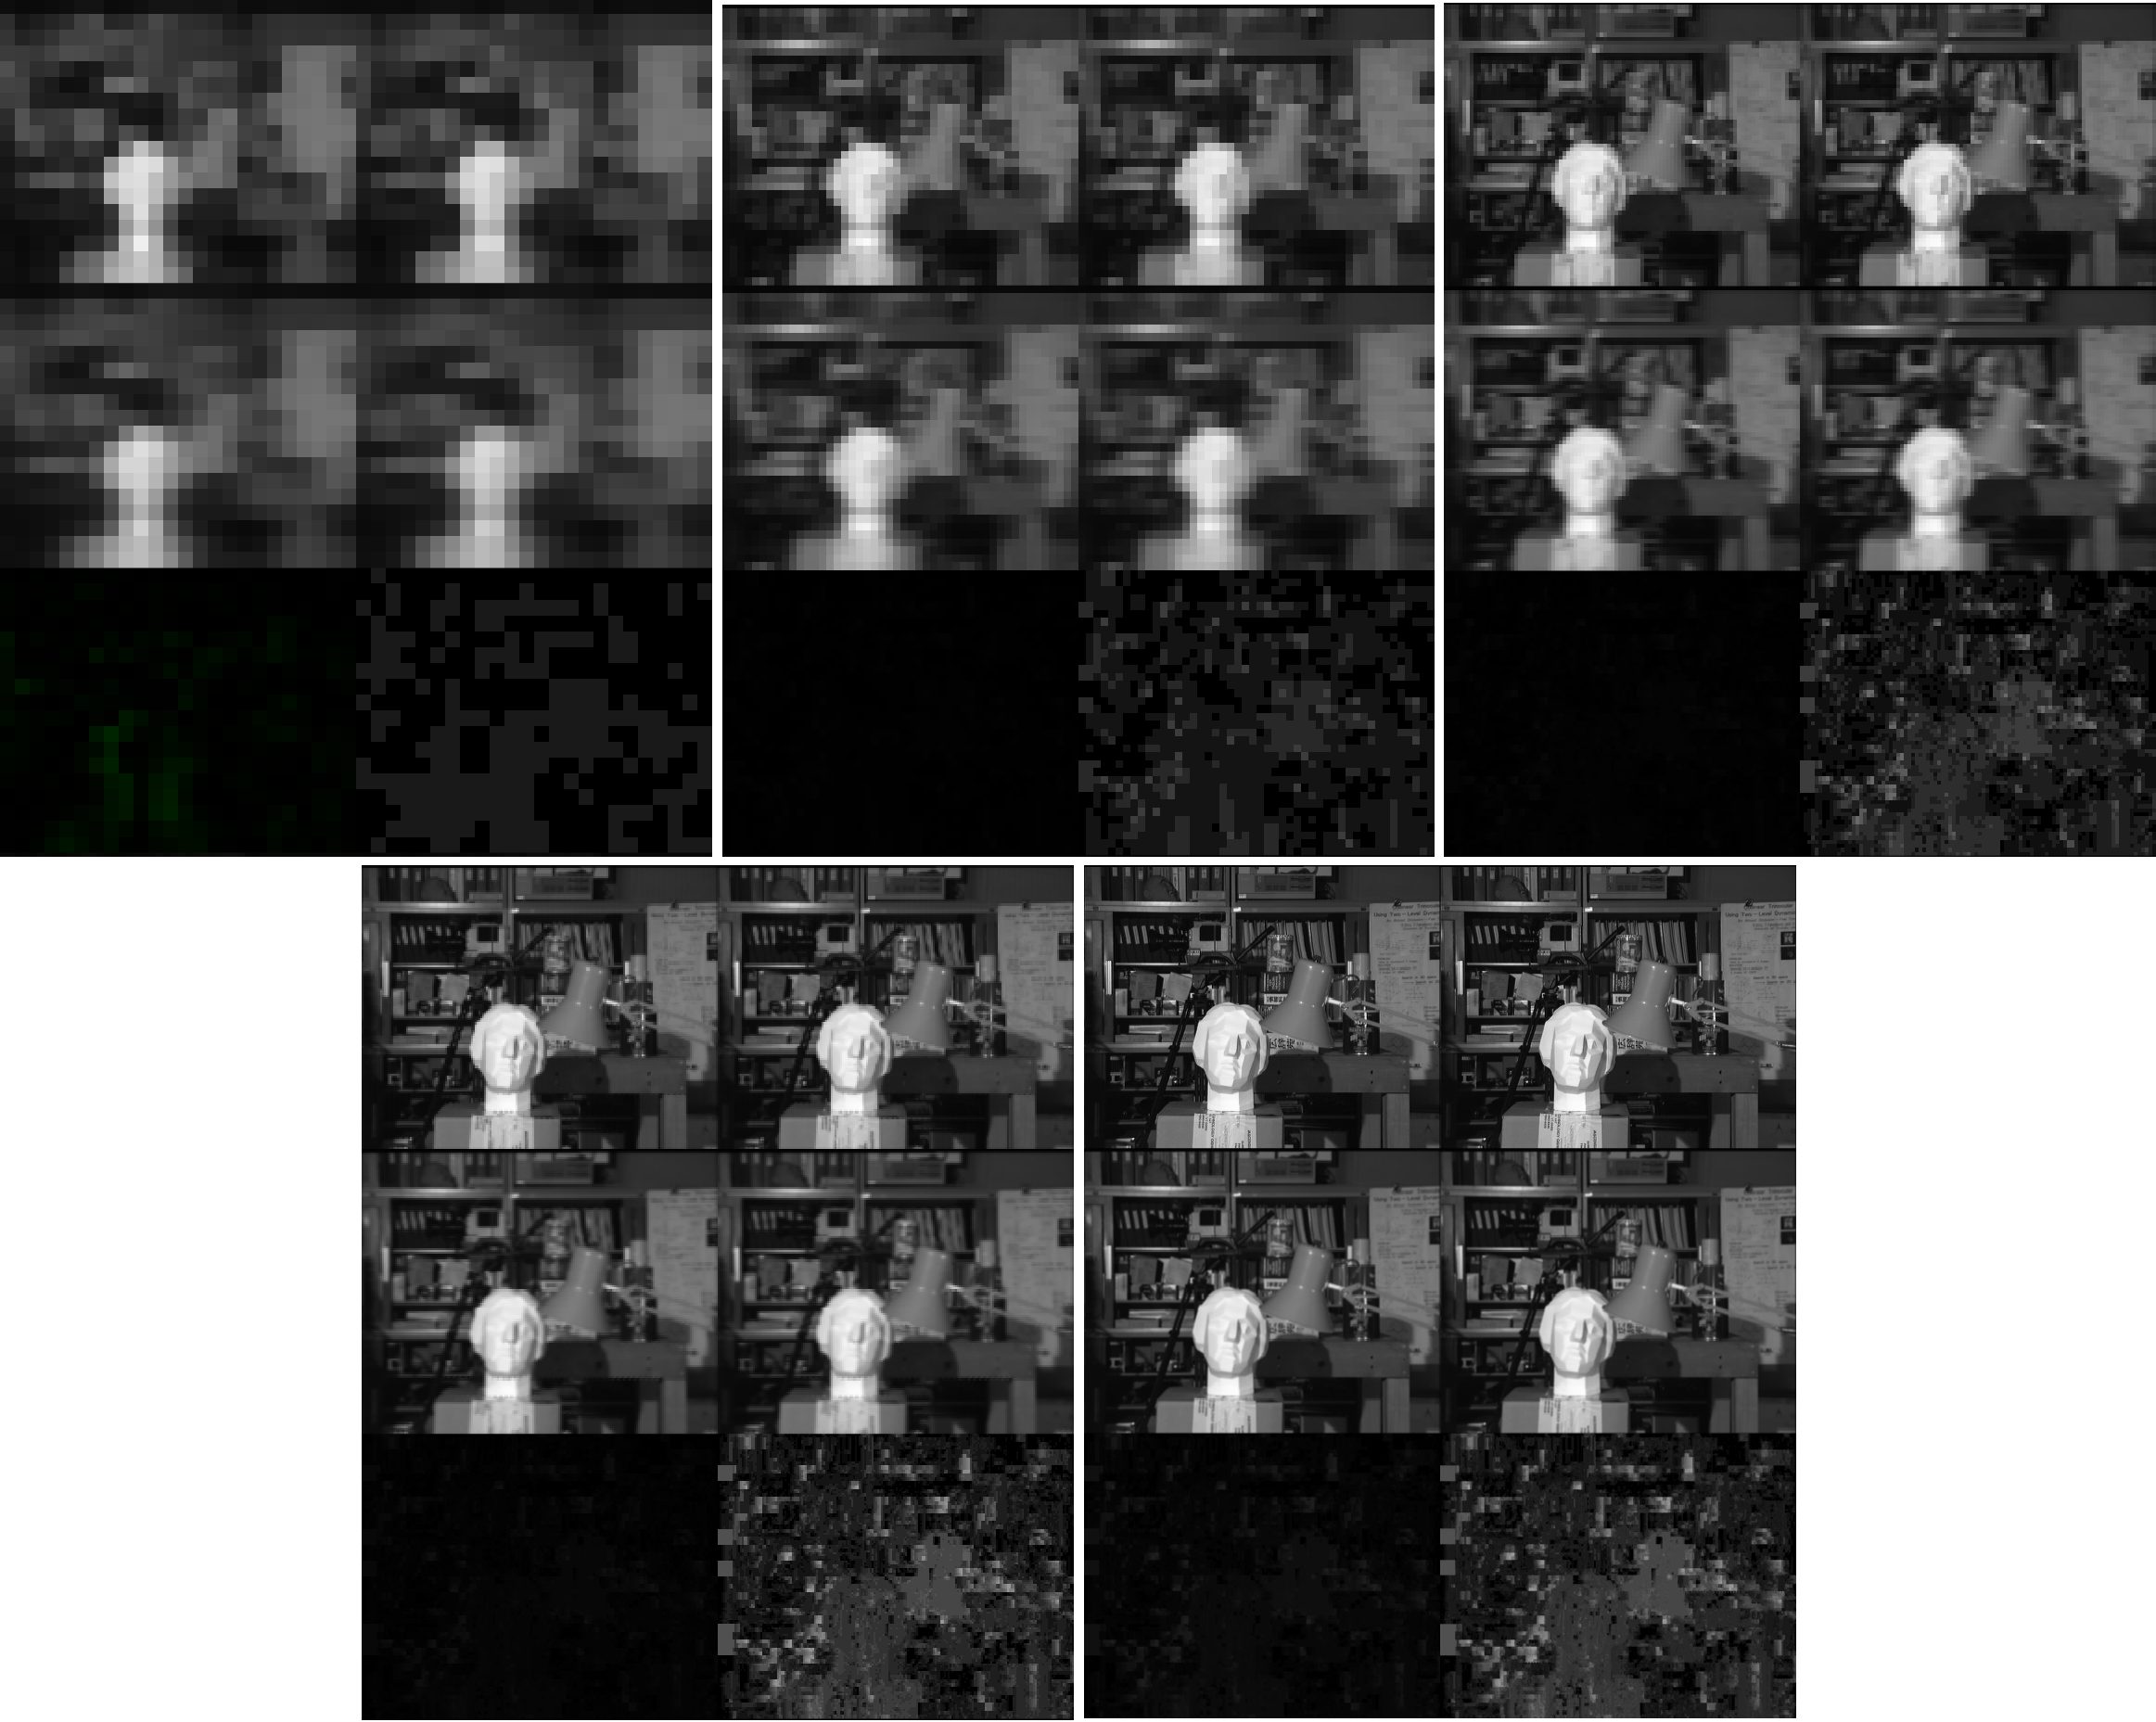
\includegraphics[width=12cm]{fig/matching1-result}\\
\caption{Tsukuba images matched on the GPU, image taken from the WebGL platform.}
\label{fig_matching1-result}
\end{center}
\end{figure}


%%%%%%%%%%%%%%%%%%%%%%%%%%%%%%%%%%%%%%%%%%%%%%%%%%%%%%%%%%%%%%%%%%%%%%
\subsubsection{Stereo-matching on GPU}
\begin{itemize}
	\item A method has been fully implemented in GPU.
	\item Results from this method are shown in figure \ref{fig/matching1-result.tex}.
\end{itemize}

%%%%%%%%%%%%%%%%%%%%%%%%%%%%%%%%%%%%%%%%%%%%%%%%%%%%%%%%%%%%%%%%%%%%%%
\subsubsection{Paper}

I am writing a paper in which I will discuss and conclude about:
\begin{itemize}
	\item GPGPU in general.
	\item GPGPU on embedded GPUs (in general and specifically through OpenGL ES 2.0).
	\item Solving the stereo matching problem on the GPU.
	\item The specifics of doing this on the Raspberry (which is a common board, but will mention other options in general).
	\item Report the results (time, accuracy) of a case study.
	\item Share code and results through the WebGL platform.
\end{itemize}
